\documentclass[conf]{new-aiaa}
%\documentclass[journal]{new-aiaa} for journal papers
\usepackage[utf8]{inputenc}

\usepackage{graphicx}
\usepackage{amsmath}
\usepackage{commath}
\usepackage[version=4]{mhchem}
\usepackage{siunitx}
\usepackage{longtable,tabularx}
\usepackage{float}
\usepackage{listings}
\usepackage{pdfpages}
\usepackage{color} %red, green, blue, yellow, cyan, magenta, black, white
\definecolor{mygreen}{RGB}{28,172,0} % color values Red, Green, Blue
\definecolor{mylilas}{RGB}{170,55,241}
\setlength\LTleft{0pt} 

\lstset{language=Matlab,%
	basicstyle=\footnotesize,
	breaklines=true,%
	morekeywords={matlab2tikz},
	keywordstyle=\color{blue},%
	morekeywords=[2]{1}, keywordstyle=[2]{\color{black}},
	identifierstyle=\color{black},%
	stringstyle=\color{mylilas},
	commentstyle=\color{mygreen},%
	showstringspaces=false,%without this there will be a symbol in the places where there is a space
	numbers=left,%
	numberstyle={\tiny \color{black}},% size of the numbers
	numbersep=9pt, % this defines how far the numbers are from the text
	emph=[1]{for,end,break},emphstyle=[1]\color{red}, %some words to emphasise
	%emph=[2]{word1,word2}, emphstyle=[2]{style},    
}

% ================================================================ % 
\title{ASE 389P.4 Methods of Orbit Determination \\ Homework 5: Setting Up the Term Project}

\author{Junette Hsin}
\affil{Masters Student, Aerospace Engineering and Engineering Mechanics, University of Texas, Austin, TX 78712}

\begin{document}

\maketitle

\begin{abstract}
	The theory and algorithms are derived and computer program to establish the trajectory of
	an Earth-orbiting satellite is developed. The assumptions for the study are:
	
	\begin{itemize}
		\item Three tracking stations taking apparent range and range-rate data are available for tracking the	satellite. Apparent quantities imply that the one-way light time between signal transmission and	reception were modeled into the measurement (i.e. the effect is dealt with).
		\item The force model used to generate the truth is the EGM96 gravity field of degree and order 20,
		attitude-dependent solar radiation pressure, and atmospheric drag.
		\item The satellite is a box-wing shaped with one Sun-pointed solar panel with known component sizes, material properties, and orientation. The spacecraft -Z axis (in the spacecraft body reference frame) is always Nadir-pointed and has the antenna.
	\end{itemize}
	

\end{abstract}


% ================================================================ % 
\section*{Problem}

% \subsubsection*{Statement} 
\begin{center}
\fbox{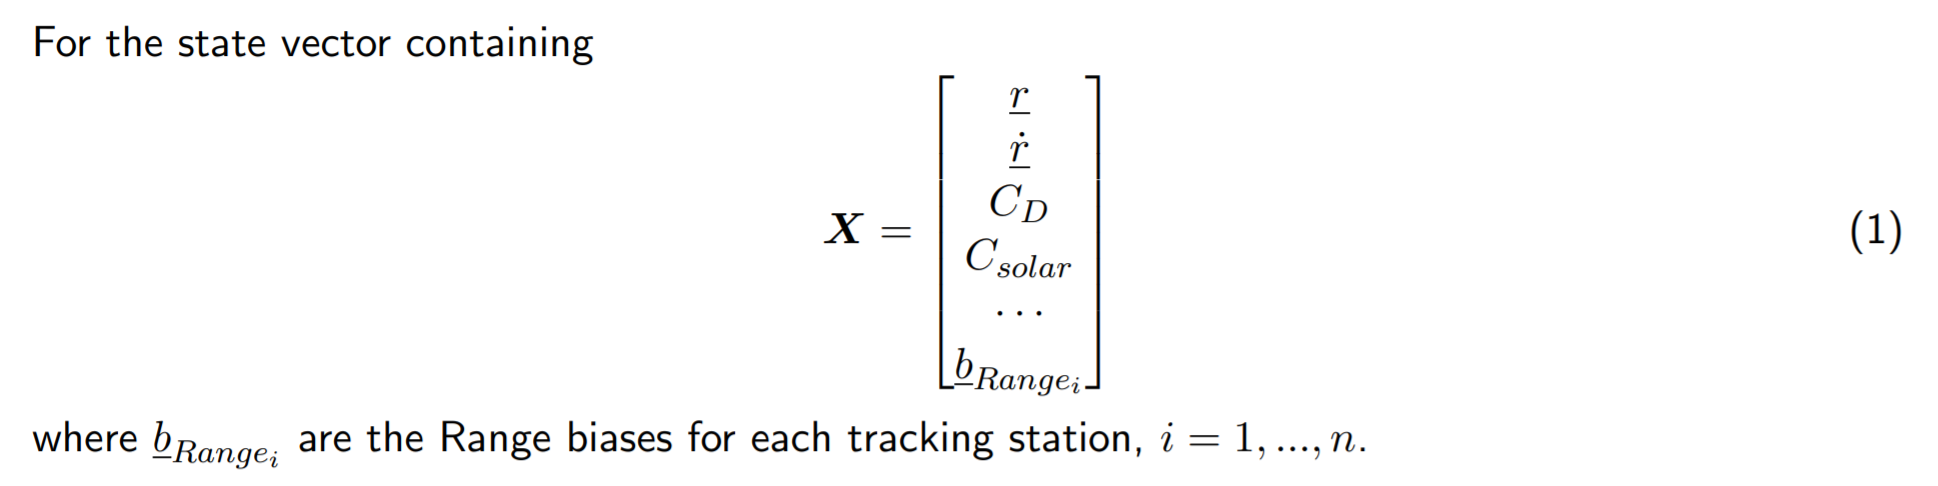
\includegraphics[width=0.9\textwidth]{prob.png}} \\
\end{center}


% ================================================================ % 
\section*{Problem 1}

 % \subsubsection*{Statement} 
\begin{center}
\fbox{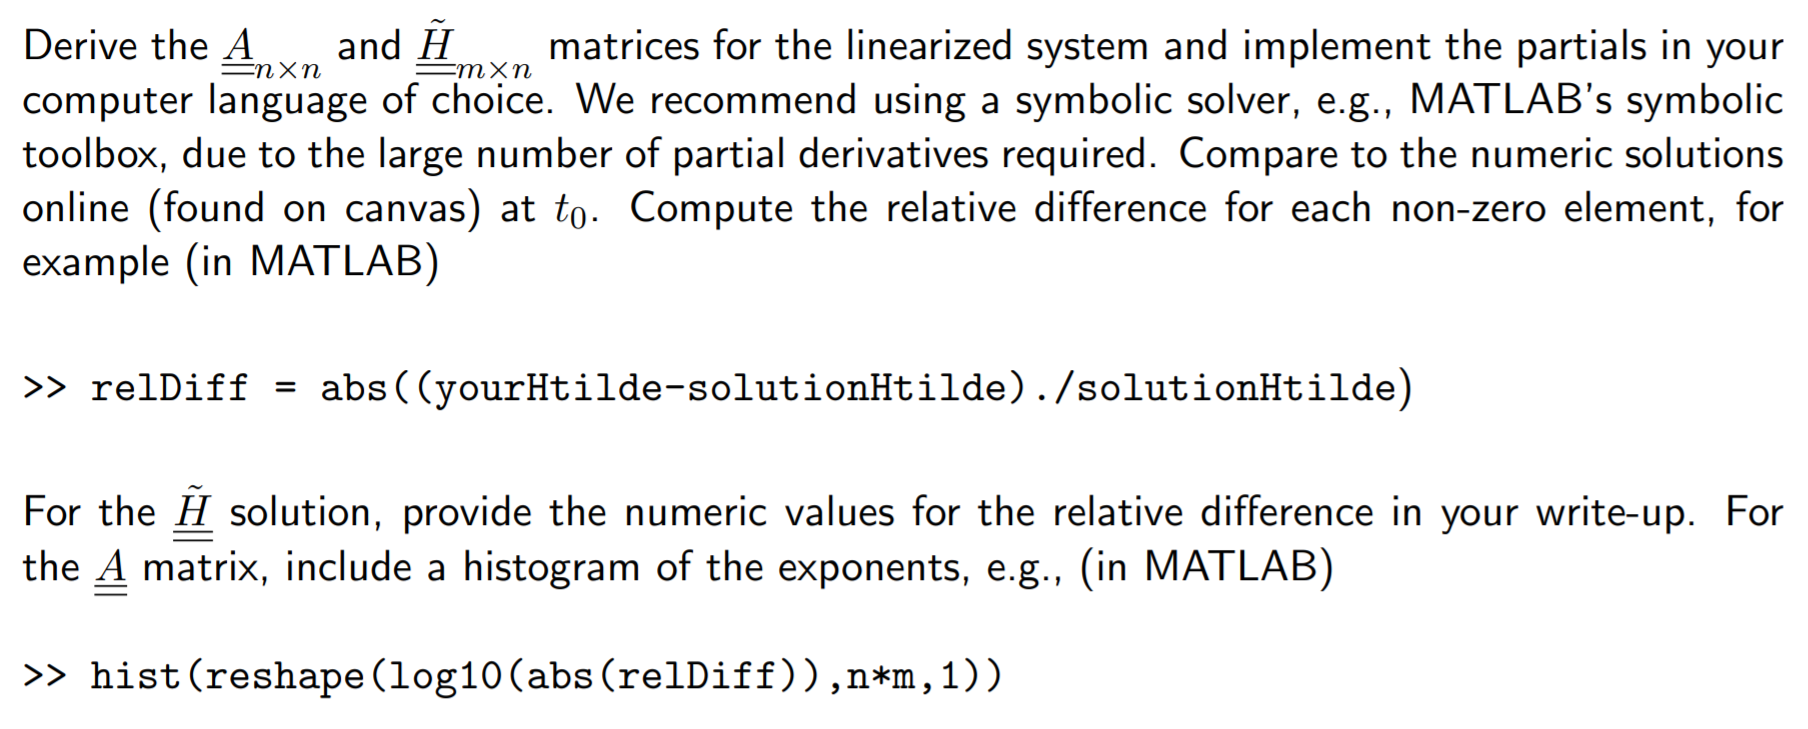
\includegraphics[width=0.9\textwidth]{prob_1.png}} \\
\end{center}

% ---------------------------------------------------------------- % 
\subsubsection*{Solution} 

\textbf{Relative difference for A matrix:}
\begin{lstlisting}
>> relDiff = abs((Ajune - Ajah)./Ajah)

relDiff =

NaN          NaN          NaN            0          NaN          NaN          NaN
NaN          NaN          NaN          NaN            0          NaN          NaN
NaN          NaN          NaN          NaN          NaN            0          NaN
3.0388e-08   2.1018e-08   1.8969e-07         1.35         1.35         1.35          1.5
3.5538e-07   6.6569e-08   6.4491e-07         1.35         1.35         1.35          1.5
7.7416e-07   1.2355e-06   1.5541e-10         1.35         1.35         1.35          1.5
NaN          NaN          NaN          NaN          NaN          NaN          NaN

\end{lstlisting}

\begin{figure}[H]
	\centering
	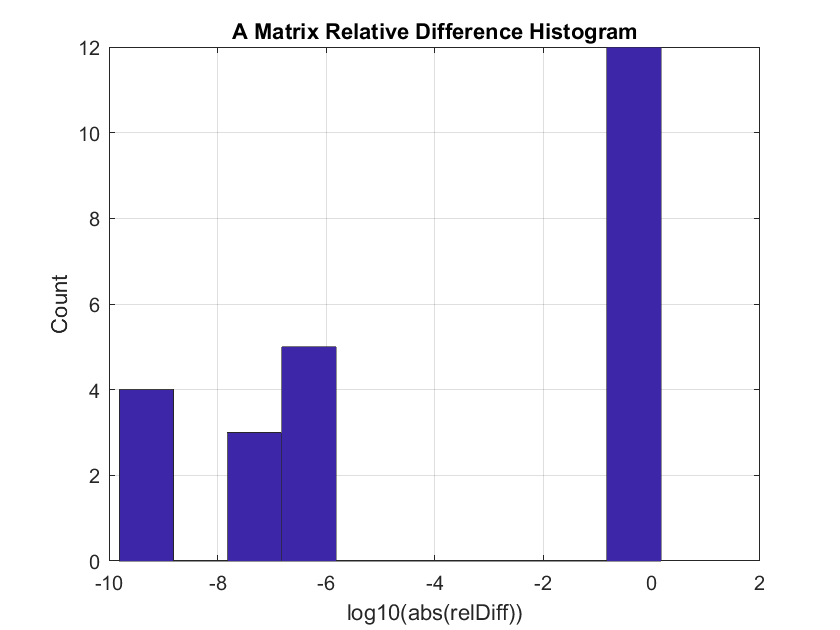
\includegraphics[width=0.8\textwidth]{prob1_A_hist.png}
\end{figure}

\textbf{Relative difference for H matrix:}
\begin{lstlisting}
>> relDiff = abs((Htjune - Htjah)./Htjah)

relDiff =

3.6195e-05    0.0011651    5.703e-06          NaN          NaN          NaN          NaN
0.053035      0.12866      0.49245   3.6195e-05    0.0011651    5.703e-06          NaN
\end{lstlisting}

\begin{figure}[H]
\centering
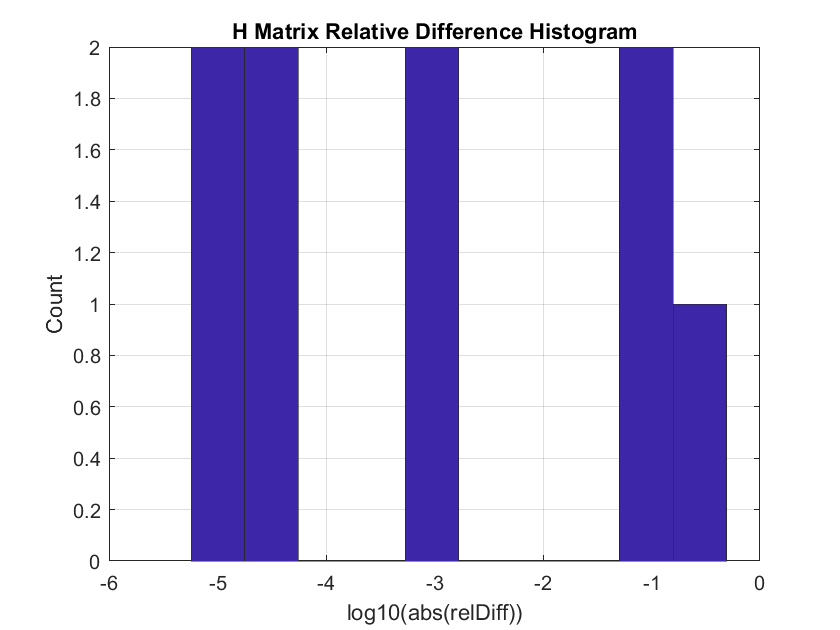
\includegraphics[width=0.8\textwidth]{prob1_H_hist.png}
\end{figure}


% ================================================================ % 
\section*{Problem 2}

% \subsubsection*{Statement} 
\begin{center}
	\fbox{
\includegraphics[width=0.9\textwidth]{prob_2.png}} \\
\end{center}

% ---------------------------------------------------------------- % 
\subsubsection*{Solution} 

\textbf{Relative difference for the end state at 21600 seconds:}
\begin{lstlisting}
>> relDiff = abs((X(end,:)' - X_GMAT)./X_GMAT)

relDiff =

0.16065
0.18772
0.20901
0.19632
0.1421
0.05198
\end{lstlisting}

\begin{figure}
\centering 
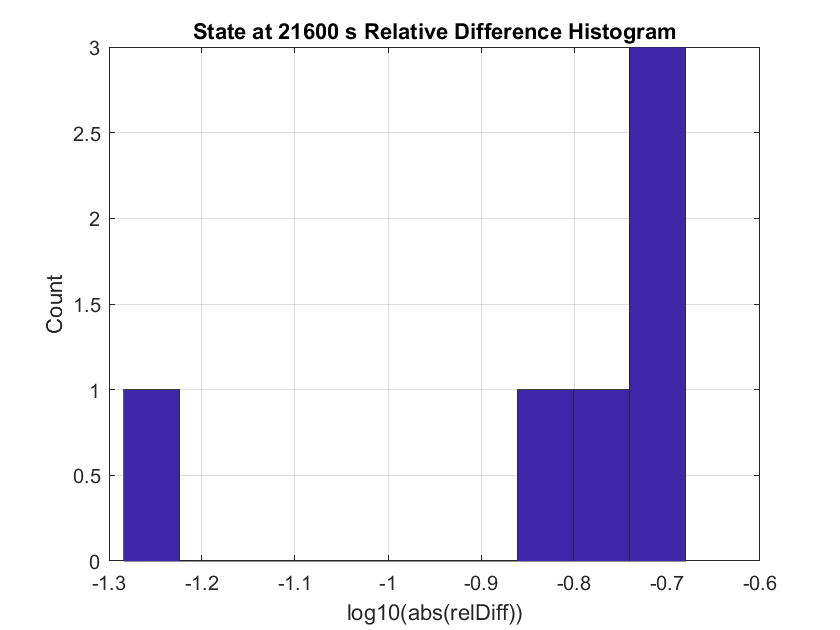
\includegraphics[width=0.8\textwidth]{prob2_state_hist.png}
\end{figure}


% ================================================================ % 
\section*{Problem 3}

% \subsubsection*{Statement} 
\begin{center}
	\fbox{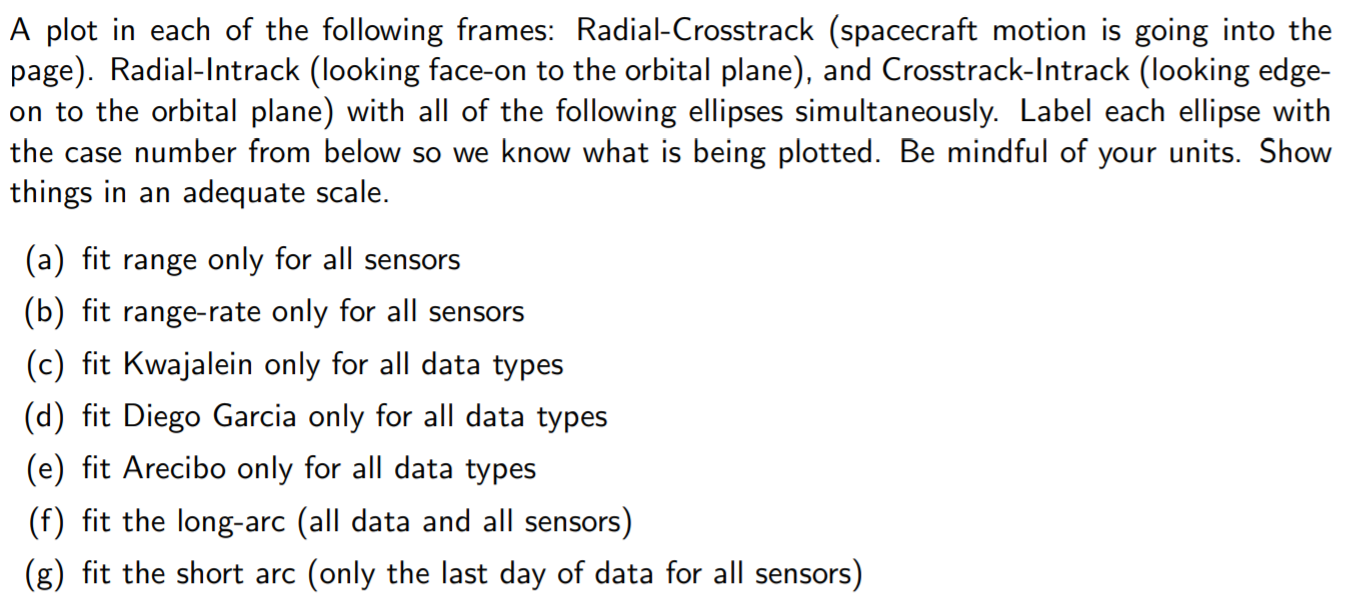
\includegraphics[width=0.9\textwidth]{prob_3.png}} \\
\end{center}

\begin{figure}
\centering 
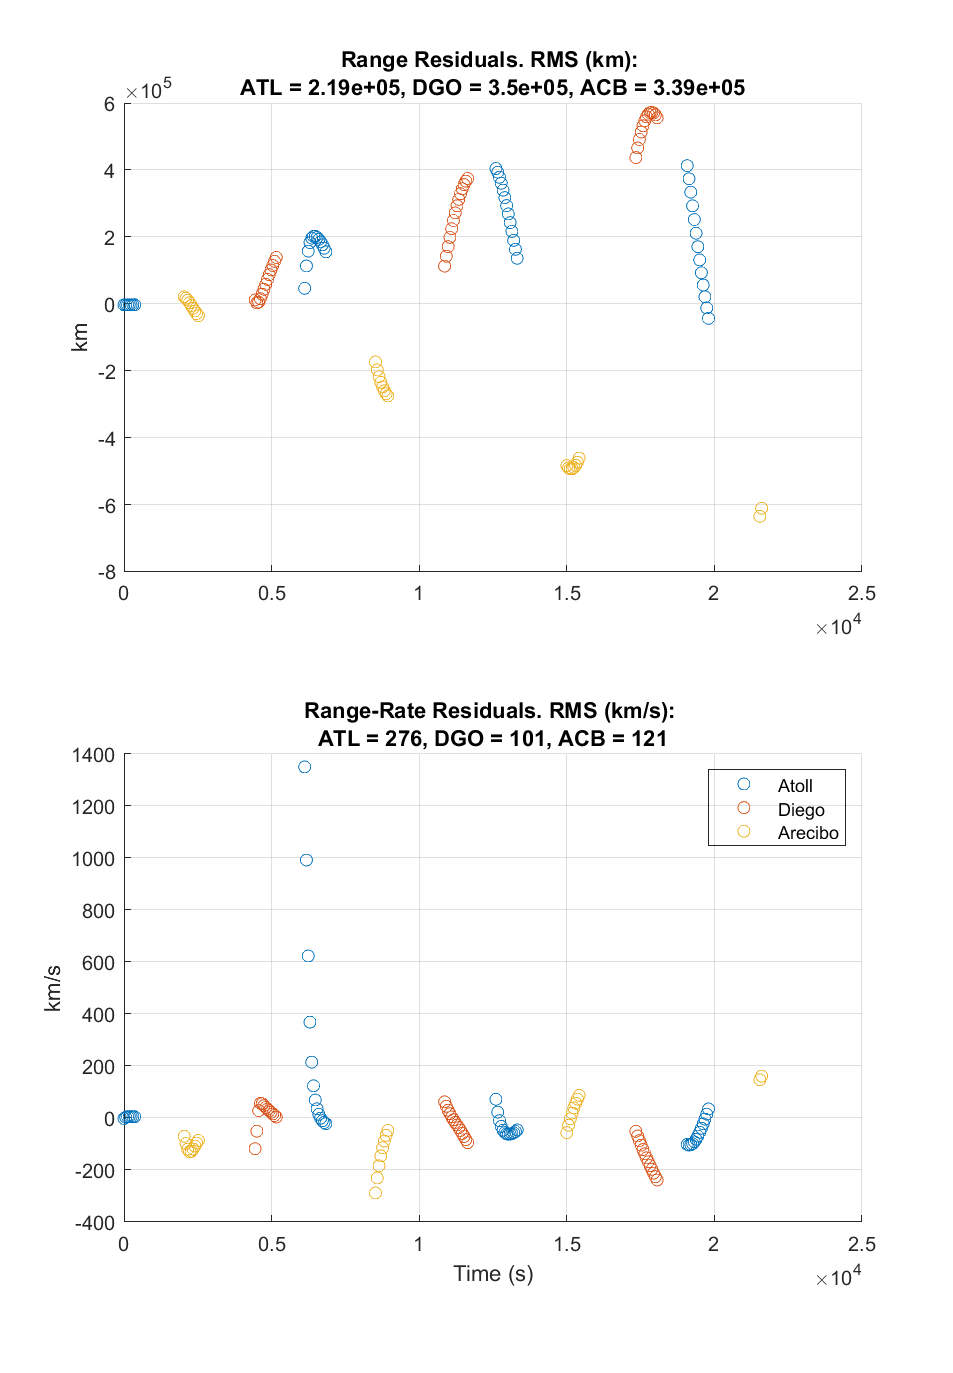
\includegraphics[width=0.8\textwidth]{range_rate_res.png}
\end{figure}

% ---------------------------------------------------------------- % 
\subsubsection*{Solution} 

The range and rate-rate residuals were calculated as the following: 

Atoll range RMS: 
\begin{lstlisting}
>> d_rms_ATL

d_rms_ATL =

2.1942e+05
\end{lstlisting}

Atoll range-rate RMS: 
\begin{lstlisting}
>> v_rms_ATL

v_rms_ATL =

275.66
\end{lstlisting}

Diego Garcia range RMS: 
\begin{lstlisting}
>> d_rms_DGO

d_rms_DGO =

3.5046e+05
\end{lstlisting}

Diego Garcia range-rate RMS: 
\begin{lstlisting}
>> v_rms_DGO

v_rms_DGO =

100.68
\end{lstlisting}

Arecibo range RMS: 
\begin{lstlisting}
>> d_rms_ACB

d_rms_ACB =

3.3891e+05
\end{lstlisting}

Arecibo range-rate RMS: 
\begin{lstlisting}
>> v_rms_ACB

v_rms_ACB =

120.98
\end{lstlisting}


\newpage
% ================================================================ % 
\section*{Appendix} 

\subsection*{HW5 MATLAB code} 

\textbf{Note: Functions to transform from ECI to ECEF and back were submitted as part of Homework 4, and so are left out of this appendix.}

\begin{lstlisting}[basicstyle=\footnotesize]
% HW 5 
% Junette Hsin 

clear; clc 
addpath(genpath('mice')); 
addpath(genpath('spice_data')); 

% Load SPICE kernel file 
cspice_furnsh( 'spice_data/naif0011.tls' )
cspice_furnsh( 'spice_data/de421.bsp' )       
cspice_furnsh( 'spice_data/pck00010.tpc ') 


%% Parameters 

% initial state initial guess (M --> KM)
CD  = 1.88; 
X0 = [ 6990.077798814194  ; 
1617.465311978378  ; 
22.679810569245355 ; 
-1.67513972506056   ; 
7.27372441330686   ; 
0.252688512916741  ; 
CD ];

% initialize STM 
STM0 = eye(7); 
STM0 = reshape(STM0, [49 1]); 
XSTM0 = [X0; STM0];  

global muE RE muS AU muM eE wE J2 J3 J4 Cd Cs eop_data 
global A m p p0 r0_drag H 

% epoch = 1 Feb 2018, 05:00:00 UTC; 
JD = 2458150.70833; 

% Constants 
muE = 398600.4415;          % Earth Gravitational Parameter (km^3/s^2) 
RE  = 6378.1363;            % Earth Radius (km)
muS = 132712440018;         % Sun's Gravitational Parameter (km^3/s^2)
AU  = 149597870.7;          % 1 Astronomical Unit (km)
muM = 4902.800066;          % Moon's Gravitational Parameter (km^3/s^2)
eE  = 0.081819221456;       % Earth's eccentricity 
wE  = 7.292115146706979e-5; % Earth's rotational velocity (rad/s)
m   = 2000;                 % satellite mass (kg) 
Cd  = 0.04;                 % diffuse reflection 
Cs  = 0.04;                 % specular reflection 

J2 = 1.08262617385222e-3; 
J3 = -2.53241051856772e-6;
J4 = -1.61989759991697e-6; 

global LEO_DATA_Apparent 
% Load observation data 
load('LEO_DATA_Apparent.mat') 

eop_data = load('finals_iau1980.txt'); 

% Atmospheric drag 
r   = norm(X0(1:3));            % km 
H   = 88667.0 / 1000;           % m --> km 
r0_drag  = (700 + RE);          % m --> km 
p0  = 3.614e-13 * 1e9;          % kg/m3 --> kg/km^3 
p   = p0*exp( -(r-r0_drag)/H ); 
A   = 15 / 1e6;                 % km^2 


%% Convert t0 to ET, i.e. seconds past J2000, the base time variable for SPICE. function calls.

%  Epoch for initial conditions 
t0      = 'Feb 1, 2018, 05:00:00 UTC'; 
abcorr  = 'NONE';

%  Convert the epoch to ephemeris time. 
et_t0   = cspice_str2et( t0 );

% extract observation epochs 
epochs = LEO_DATA_Apparent(:,2); 
epochs = et_t0 + epochs; 


%% Derive A matrix 

X  = sym('X', [7 1]); 
dX = fn.EOM(et_t0, X); 

% compute partials 
Amat    = jacobian( dX, X );       
Amat_fn = matlabFunction(Amat); 

% test Amat_fn at t0 
Ajune = Amat_fn( X0(1), X0(2), X0(3), X0(4), X0(5), X0(6), X0(7))   ; 
Ajah  = load('A_t0.mat'); Ajah = Ajah.A; 

disp('Ajah ./ Ajune: ')
disp(Ajah ./ Ajune); 


%% integrate EOM 

% set ode45 params 
rel_tol = 1e-10;         % 1e-14 accurate; 1e-6 coarse 
abs_tol = 1e-10; 
options = odeset('reltol', rel_tol, 'abstol', abs_tol ); 

% Set run state 
run_state = 2; 
disp('Running sim ...') 

if run_state == 1
% fuck the STM for now. integrate 
[t, X] = ode45(@fn.EOM, [epochs(1) : 60 : epochs(end)], X0, options); 
elseif run_state == 2
[t, XSTM] = ode45(@(t, XSTM) fn.EOM_STM(t, XSTM, Amat_fn), [epochs(1) : 60 : epochs(end)], XSTM0, options); 
X = XSTM(:, 1:6); 
end 
disp('Pos and Vel end: ')
disp(X(end, 1:6)'); 

%% Plot what u see 

% create figure 
ftitle = 'Orbit'; 
figure('name', ftitle);  

r_x = X(:,1); r_y = X(:,2); r_z = X(:,3); 
plot3(r_x, r_y, r_z); hold on; grid on; 
scatter3(r_x(1), r_y(1), r_z(1)); 
scatter3(r_x(end), r_y(end), r_z(end), 'kx'); 
xlabel('x (LU)'); ylabel('y (LU)'); zlabel('z (LU)'); 
title(ftitle)

ftitle = 'A Matrix Relative Difference Histogram'; 
figure('name', ftitle); 
relDiff = abs((Ajune - Ajah)./Ajah); 
hist(reshape(log10(abs(relDiff)),7*7,1)); 
title('A Matrix Relative Difference Histogram') 
ylabel('Count') 
xlabel('log10(abs(relDiff))') 

% Compare with solution 
X_GMAT = [
-5153.790483
-4954.421472
-144.8250293
5.178059443
-5.38748629
-0.211928207]; 

ftitle = 'State at 21600 s Relative Difference Histogram'; 
figure('name', ftitle); 
relDiff = abs((X(end,:)' - X_GMAT)./X_GMAT); 
hist(log10(abs(relDiff))); 
title(ftitle) 
ylabel('Count') 
xlabel('log10(abs(relDiff))') 


%% Convert coordinates ECEF <--> ECI 

global eopdata const

SAT_Const

% read Earth orientation parameters
fid = fopen('eop19620101.txt','r');
%  ----------------------------------------------------------------------------------------------------
% |  Date    MJD      x         y       UT1-UTC      LOD       dPsi    dEpsilon     dX        dY    DAT
% |(0h UTC)           "         "          s          s          "        "          "         "     s 
%  ----------------------------------------------------------------------------------------------------
eopdata = fscanf(fid,'%i %d %d %i %f %f %f %f %f %f %f %f %i',[13 inf]);
fclose(fid);

% Station coords. Convert M --> KM 
r_ATL_ECEF = [-6143584  1364250  1033743]' / 1000;  % Atoll 
r_DGO_ECEF = [ 1907295  6030810 -817119 ]' / 1000;  % Diego 
r_ACB_ECEF = [ 2390310 -5564341  1994578]' / 1000;  % Arecibo 
v_ATL_ECEF = [0; 0; 0]; 
v_DGO_ECEF = [0; 0; 0]; 
v_ACB_ECEF = [0; 0; 0]; 

JD_UTC     = cspice_et2utc(et_t0, 'J', 10); 
JD_UTC     = str2num(extractAfter(JD_UTC, 'JD ')); 

% Convert to ECI frame 
r_ATL_ECI  = fn.ECEFtoECI(JD, r_ATL_ECEF); 
v_ATL_ECI  = v_ATL_ECEF + cross([ 0 0 wE ]', r_ATL_ECEF); 
v_ATL_ECI  = fn.ECEFtoECI(JD, v_ATL_ECI); % Technically wrong. Look in Vallado 

v_ATL_ECI  = fn.ECEFtoECI(JD, v_ATL_ECEF) + cross([ 0 0 wE]', r_ATL_ECEF); 

r_DGO_ECI  = fn.ECEFtoECI(JD, r_DGO_ECEF); 
v_DGO_ECI  = v_ATL_ECEF + cross([ 0 0 wE ]', r_DGO_ECEF); 
v_DGO_ECI  = fn.ECEFtoECI(JD, v_DGO_ECI); % Technically wrong. Look in Vallado 

r_ACB_ECI  = fn.ECEFtoECI(JD, r_ACB_ECEF); 
v_ACB_ECI  = v_ATL_ECEF + cross([ 0 0 wE ]', r_ACB_ECEF); 
v_ACB_ECI  = fn.ECEFtoECI(JD, v_ACB_ECI); % Technically wrong. Look in Vallado 

% KM 
r0_ECEF = fn.ECItoECEF(JD, [X0(1) X0(2) X0(3)]'); 
v0_ECEF = X0(4:6) + cross([ 0 0 -wE ]', [X0(1) X0(2) X0(3)]'); 
X0_ECEF = [r0_ECEF; v0_ECEF]; 


% %% Mahooti check 
% 
% MJD_UTC    = JD_UTC - 2400000.5; 
% 
% % Atoll 
% Y          = ECEF2ECI(MJD_UTC, [r_ATL_ECEF; v_ATL_ECEF]'); 
% r_ATL_ECI  = Y(1:3); 
% v_ATL_ECI  = Y(4:6); 
% 
% % Diego
% Y          = ECEF2ECI(MJD_UTC, [r_DGO_ECEF; v_DGO_ECEF]'); 
% r_DGO_ECI  = Y(1:3); 
% v_DGO_ECI  = Y(4:6); 
% 
% % Arecibo 
% Y          = ECEF2ECI(MJD_UTC, [r_ACB_ECEF; v_ACB_ECEF]'); 
% r_ACB_ECI  = Y(1:3); 
% v_ACB_ECI  = Y(4:6); 


%% DO EVERYTHING IN ECI FRAME 

X = sym('X', [7; 1]); 

% Atoll 
XS = [ r_ATL_ECI; v_ATL_ECI ]; 
Ht_ATL_fn = fn.Ht_fn(XS); 

% Diego 
XS = [ r_DGO_ECI; v_DGO_ECI ]; 
Ht_DGO_fn = fn.Ht_fn(XS); 

% Arecibo 
XS = [ r_ACB_ECI; v_ACB_ECI ]; 
Ht_ACB_fn = fn.Ht_fn(XS); 

X0_H   = X0; 
Htjune = Ht_ATL_fn( X0_H(1), X0_H(2), X0_H(3), X0_H(4), X0_H(5), X0_H(6))   ; 
Htjah  = load('H_Tilde_t0.mat'); Htjah = Htjah.H_TILDA; 

disp('Htjune: ')
disp(Htjune)
disp('Htjah: ') 
disp(Htjah)
disp('Htjune - Htjah: ')
disp(Htjune - Htjah)

ftitle = 'H Matrix Relative Difference Histogram'; 
figure('name', ftitle); 
relDiff = abs((Htjune - Htjah)./Htjah); 
hist(reshape(log10(abs(relDiff)),2*7,1)); 
title('H Matrix Relative Difference Histogram') 
ylabel('Count') 
xlabel('log10(abs(relDiff))') 


%% Calculate residuals 

% Reset t to start incrementing at 0 
t_XSTM = t - t(1); 

% Atoll 
[t_ATL, d_err_ATL, d_rms_ATL, v_err_ATL, v_rms_ATL] = ... 
fn.Y_residuals(1, t_XSTM, XSTM, Ht_ATL_fn); 

% Diego 
[t_DGO, d_err_DGO, d_rms_DGO, v_err_DGO, v_rms_DGO] = ... 
fn.Y_residuals(2, t_XSTM, XSTM, Ht_DGO_fn); 

% Arecibo 
[t_ACB, d_err_ACB, d_rms_ACB, v_err_ACB, v_rms_ACB] = ... 
fn.Y_residuals(3, t_XSTM, XSTM, Ht_ACB_fn); 

ftitle = 'Residuals'; 
figure('name', ftitle); 
subplot(2,1,1) 
scatter(t_ATL, d_err_ATL); hold on; grid on; 
scatter(t_DGO, d_err_DGO); 
scatter(t_ACB, d_err_ACB); 
title({'Range Residuals. RMS (km): '; ... 
	sprintf('ATL = %.3g, DGO = %.3g, ACB = %.3g', d_rms_ATL, d_rms_DGO, d_rms_ACB) }); 
	ylabel('km')  
	subplot(2,1,2) 
	scatter(t_ATL, v_err_ATL); hold on; grid on; 
	scatter(t_DGO, v_err_DGO); 
	scatter(t_ACB, v_err_ACB); 
	title({'Range-Rate Residuals. RMS (km/s): '; ... 
		sprintf('ATL = %.3g, DGO = %.3g, ACB = %.3g', v_rms_ATL, v_rms_DGO, v_rms_ACB) }); 
		xlabel('Time (s)') 
		ylabel('km/s') 
		legend('Atoll', 'Diego', 'Arecibo', 'color', 'none');
\end{lstlisting}

\subsubsection{EOM}
\begin{lstlisting}
function dX = EOM(et, X)
% ------------------------------------------------------------------------
% Purpose: Generate EOM for satellite orbiting earth due to geopotential,
% lunisolar, SRP, and drag perturbations 
% 
% Inputs 
%   t   = [1x1] time (ET epoch) vector 
%   X   = [7x1] state vector in ECI frame (inertial) 
% 
% Outputs 
%   dX  = [7x1] derivative of state vector 
% ------------------------------------------------------------------------

global wE muE 
global A m p0 r0_drag H  

% force column vector. Check if X is numeric or symbolic 
if isnumeric(X)
dX = zeros(7, 1);   
else 
dX = sym(zeros(7,1)); 
end

% Set velocity and CD 
dX(1:3) = X(4:6);
CD = X(7); 

% accel due to point mass (not needed when geopotential gravity is present)
r       = norm(X(1:3)); 
% dX(4:6) = ( - muE / r^3 ) * X(1:3); 

% accel due to gravity
% if isnumeric(X); g = fn.a_spherical(et, X); else g = fn.g_J2J3J4(X); end
% g = fn.a_spherical(et, X); 
g = fn.g_J2J3J4(X); 
dX(4:6) = dX(4:6) + g; 

% accel due to lunisolar perturbation 
[a_sun, a_moon] = fn.lunisolar(et, X); 
dX(4:6) = dX(4:6) + a_sun + a_moon; 

% accel due to SRP 
a_srp   = fn.a_SRP(et, X); 
dX(4:6) = dX(4:6) + a_srp; 

% CHECK UNITS. USE KM !!!
% accel due to drag 
pA      = p0 * exp( -(r - r0_drag)/H ); 
VA      = X(4:6) - cross( [0; 0; wE], X(1:3) ); 
VAnorm  = norm(VA); 
a_drag  = - 1/2 * CD * A/m * pA * VAnorm * VA;
% a_drag  = a_drag / 26.5;  % Correct to match Jah's Amat??? 
dX(4:6) = dX(4:6) + a_drag; 

end 
\end{lstlisting}

\subsubsection{EOM\_STM}
\begin{lstlisting}
function dX = EOM_STM(et, X, Amat_fn)
% ------------------------------------------------------------------------
% Purpose: Generate EOM for satellite orbiting earth due to gravity (EGM 96),
% lunisolar perturbations, SRP, and drag 
% 
% Inputs 
%   t   = [7x1] time (ET epoch) vector 
%   rv  = [49x1] state vector in ECI frame (inertial) 
% 
% Outputs 
%   drv = [49x1] derivative of state vector 
% ------------------------------------------------------------------------

% force column vector 
dX = zeros(7+49, 1);   

% EOM 
dX(1:7) = fn.EOM(et, X); 

% STM stuff 
Amat = Amat_fn(X(1), X(2), X(3), X(4), X(5), X(6), X(7)); 
STM  = X(8:7+49); 
STM  = reshape(STM, [7 7]); 
dSTM = Amat*STM; 
dSTM = reshape(dSTM, [49,1]); 

dX(8:7+49) = dSTM; 

end 
\end{lstlisting}

\subsubsection{Ht\_fn}
\begin{lstlisting}
function Ht_fn_out = Ht_fn(XS)

X = sym('X', [7; 1]); 

r_site = [X(1)-XS(1); X(2)-XS(2); X(3)-XS(3)]; 
v_site = [X(4)-XS(4); X(5)-XS(5); X(6)-XS(6)]; 
d      = norm(r_site); 
v      = dot(v_site, r_site/norm(r_site)); 

Htmat      = sym(zeros(2,7)); 
Htmat(1,:) = simplify(gradient(d, X)); 
Htmat(2,:) = simplify(gradient(v, X)); 
Ht_fn_out  = matlabFunction(Htmat); 

end 
\end{lstlisting}

\subsubsection{Y\_residuals}
\begin{lstlisting}
function [t_STA, d_err_STA, d_rms_STA, v_err_STA, v_rms_STA] = ... 
Y_residuals(ID_STA, t_XSTM, XSTM, Ht_STA_fn)

global LEO_DATA_Apparent 

% Station data 
i_STA     = find(LEO_DATA_Apparent(:, 1) == ID_STA); 
Yobs_STA  = LEO_DATA_Apparent(i_STA, :); 
t_STA     = Yobs_STA(:, 2); 

% Calculate Y = H * x 
Ycalc_STA = zeros(size(Yobs_STA)); 
Ycalc_STA(:, 1:2) = Yobs_STA(:, 1:2); 
for i = 1:length(i_STA) 

% find t index 
ti    = Yobs_STA(i,2); 
i_XSTM = find(t_XSTM == ti); 

% Extract states 
Xi   = XSTM( i_XSTM, 1:7)'; 
STMi = XSTM( i_XSTM, 8:7+49 ); 
STMi = reshape(STMi, [7 7]); 

% compute H 
Hti = Ht_STA_fn(Xi(1), Xi(2), Xi(3), Xi(4), Xi(5), Xi(6)) * STMi; 

% Y = H * x
Ycalc_STA(i,3:4) = Hti * Xi; 

end 

% Calculate residuals 
d_err_STA = Yobs_STA(:,3) - Ycalc_STA(:,3); 
d_rms_STA = rms(d_err_STA); 
v_err_STA = Yobs_STA(:,4) - Ycalc_STA(:,4); 
v_rms_STA = rms(v_err_STA); 

end 
\end{lstlisting}





% ================================================================ % 

\bibliography{sample}

\end{document}
